\documentclass[a4paper,12pt,portuguese]{report}
\usepackage[utf8]{inputenc}
\usepackage[portuguese]{babel}
\usepackage{ragged2e}
\usepackage{fancyvrb}
\usepackage{graphicx}

\title{Projeto do grupo 40 \\Programação Orientada aos Objectos}
\author{Martins, José(a78821)\
        \and
        Costa, Mariana(a78824)\
        \and
        Quaresma, Miguel(a77049)
        }
\date{\today}

\begin{document}
 
\begin{titlepage}
\maketitle
\end{titlepage}
 
\tableofcontents
 
\chapter{Introdução}


\chapter{Desenvolvimento}

\section{Classes}

\begin{figure}[ht!]
    \centering
        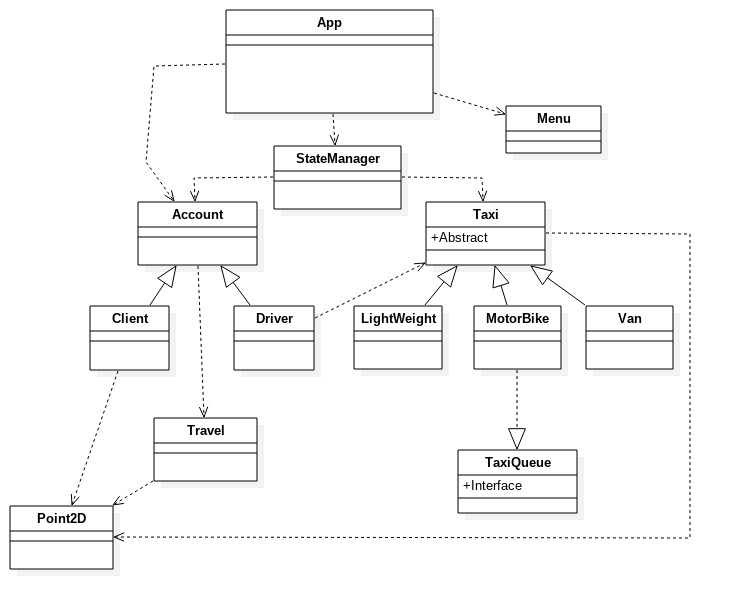
\includegraphics[width=120mm]{graph.jpg}
    \caption{Principais Classes}
\end{figure}

Em termos de classes, como podemos visualizar na imagem acima, temos uma cla    sse principal(App) que "controla" tudo, dependendo por composição das classes StateManager, Account e Menu.

\chapter{Conclusão}

\end{document}
